\chapter{Application Architecture}
\section{Overview}
This chapter describes application architecture which was purpose of this thesis. Application is organized into \textbf{four} essential parts:
\begin{itemize}
	\item Data source: loadstone DBMS
	\item Module 1: loadstone-model
	\item Module 2: loadstone-api
	\item Module 3: loadstone-package
\end{itemize}

\textit{Note: naming convention can differ from standard UML definitions. Module can be considered as component - represents a modular part of a system, that encapsulates its content and whose manifestation is replaceable within its environment. A component defines its behavior in terms of provided and required interfaces\cite{22}. Module convention comes from the fact that application lifecycle and dependency management is used by tool \textbf{Maven}. Maven uses naming convention of modules and helps developer to avoid introducing circular dependencies so application is easier to maintain in future \cite{23}.}

\section{Architecture scheme}
In the figure \ref{fig:@=architecture} is depicted overall architecture of loadstone application.
\begin{figure}
	\centering
	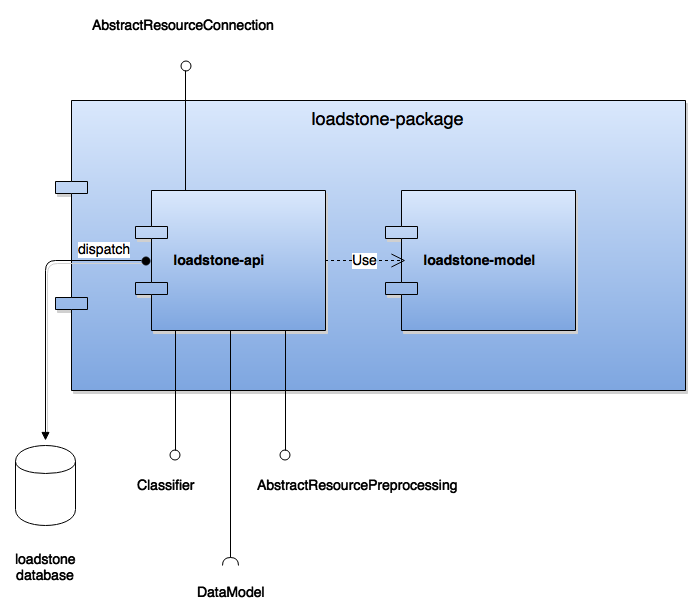
\includegraphics[scale=0.6]{architecture.png}
	\caption{Loadstone application architecture}
	\label{fig:@=architecture}
\end{figure}

\section{Architecture UML Class diagram}
To explore more implementation of application there is a figure \ref{fig:@=loadstone_uml} which clearly describes technical details of application.
\begin{figure}
	\centering
	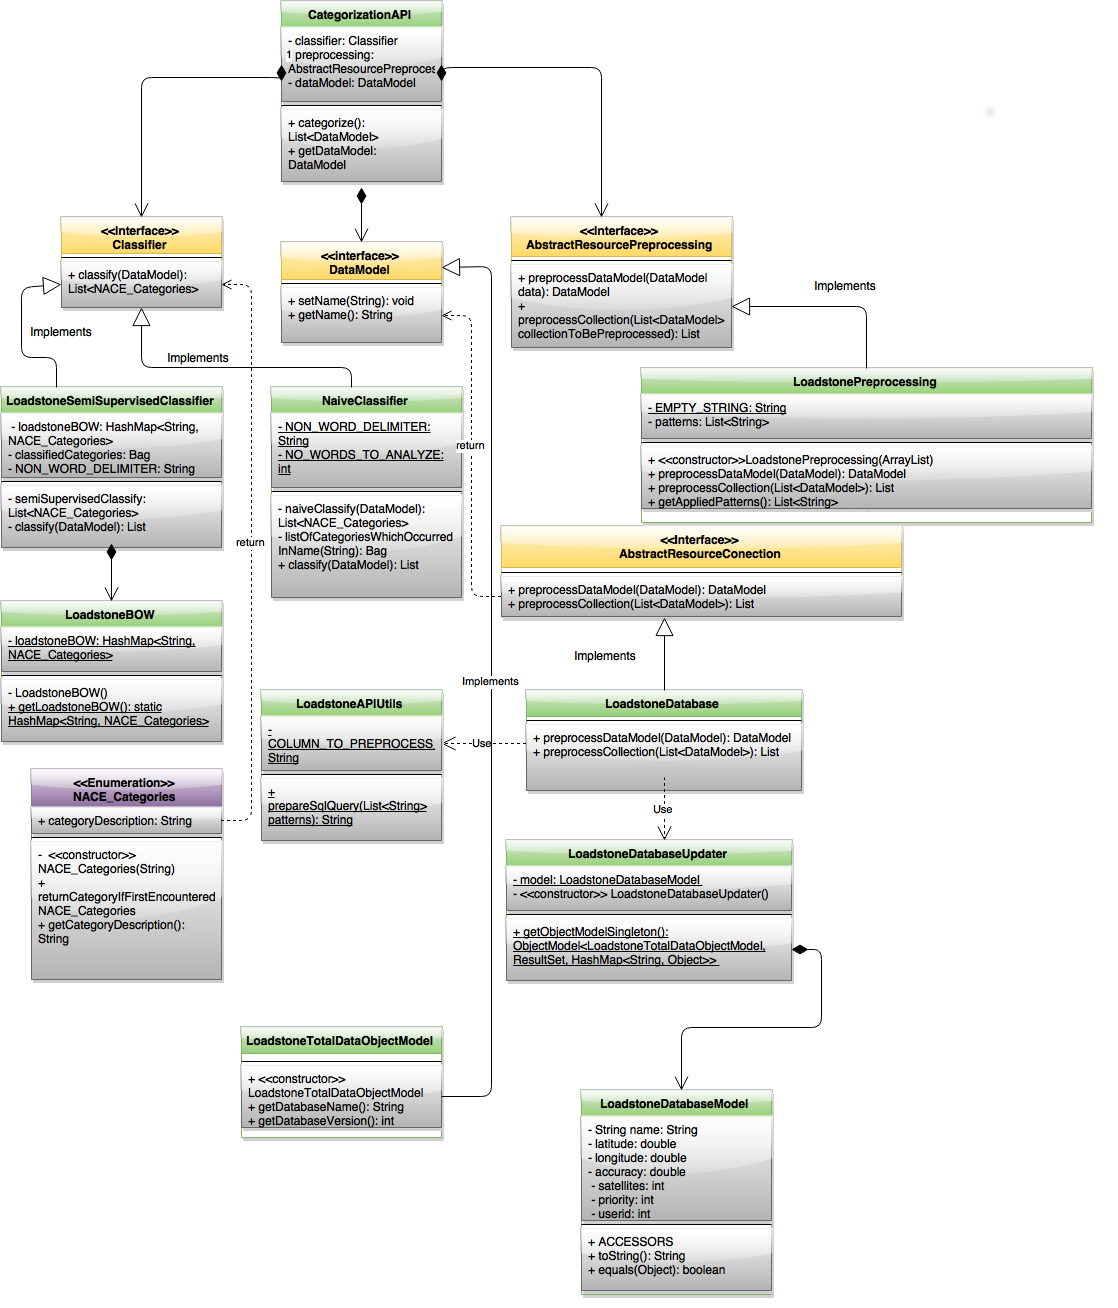
\includegraphics[scale=0.4]{UML.png}
	\caption{Loadstone application UML Class Diagram}
	\label{fig:@=loadstone_uml}
\end{figure}
